% Ty Stanford
% 2016-02-11

\documentclass{beamer}

\usepackage{tikz}
\usepackage{amssymb}
\usepackage{fancyvrb}
\usepackage{color, colortbl}
\usepackage[utf8]{inputenc}
\usepackage[scaled=.8]{beramono}
\usepackage[T1]{fontenc}
\usepackage{mathrsfs}


% Set themes like Madrid or Szeged or Warsaw (are the best)
% AnnArbor is also good, add yellow to the current theme/colour theme
% see: https://www.hartwork.org/beamer-theme-matrix/
%\usetheme{Szeged} 

% can also set the colour theme:
% default=blue, beaver=red, seagull=grey, 
\usecolortheme{beaver}


\setbeamertemplate{navigation symbols}{}


\definecolor{lghtGrey}{gray}{0.9}
\definecolor{lghtGreytwo}{gray}{0.65}

\definecolor{darkredpurple}{rgb}{0.243,0.082,0.165}
\definecolor{lightmaroon1}{rgb}{0.451,0.086,0.188}
\definecolor{lightmaroon2}{rgb}{0.851,0.392,0.290}
\definecolor{pinkoffwhite}{rgb}{0.950,0.869,0.753}
\definecolor{midgrey1}{rgb}{0.220,0.220,0.251}
\definecolor{midgrey2}{rgb}{0.7,0.7,0.7}
\definecolor{darkblue1}{rgb}{0.1,0.1,0.6}
\definecolor{aublue}{rgb}{0.157,0.322,0.614}
\definecolor{linkblue}{rgb}{0.192,0.494,0.675}


%\setbeamercolor{alerted text}{fg=orange}
%\setbeamercolor{background canvas}{bg=white}
%\setbeamercolor{block body alerted}{bg=normal text.bg!90!black}
\setbeamercolor{block body}{bg=pinkoffwhite!80}
%\setbeamercolor{block body}{bg=normal text.bg!90!black}
%\setbeamercolor{block body example}{bg=normal text.bg!90!black}
%\setbeamercolor{block title alerted}{use={normal text,alerted text},fg=alerted text.fg!75!normal text.fg,bg=normal text.bg!75!black}
%\setbeamercolor{block title}{bg=lightmaroon1!10}
%\setbeamercolor{block title example}{use={normal text,example text},fg=example text.fg!75!normal text.fg,bg=normal text.bg!75!black}
%\setbeamercolor{fine separation line}{}
%\setbeamercolor{frametitle}{fg=brown}
%\setbeamercolor{item projected}{fg=black}
%\setbeamercolor{normal text}{bg=black,fg=yellow}
%\setbeamercolor{palette sidebar primary}{use=normal text,fg=normal text.fg}
%\setbeamercolor{palette sidebar quaternary}{use=structure,fg=structure.fg}
%\setbeamercolor{palette sidebar secondary}{use=structure,fg=structure.fg}
%\setbeamercolor{palette sidebar tertiary}{use=normal text,fg=normal text.fg}
%\setbeamercolor{section in sidebar}{fg=brown}
%\setbeamercolor{section in sidebar shaded}{fg=grey}
%\setbeamercolor{separation line}{}
%\setbeamercolor{sidebar}{bg=red}
%\setbeamercolor{sidebar}{parent=palette primary}
%\setbeamercolor{structure}{bg=black, fg=green}
%\setbeamercolor{subsection in sidebar}{fg=brown}
%\setbeamercolor{subsection in sidebar shaded}{fg=grey}
%\setbeamercolor{title}{fg=brown}
%\setbeamercolor{titlelike}{fg=brown}



%\setbeamercolor*{palette primary}{fg=pinkoffwhite}
%\setbeamercolor*{palette secondary}{fg=pinkoffwhite}
%\setbeamercolor*{palette tertiary}{bg=pinkoffwhite}
\setbeamercolor{frametitle}{fg=lightmaroon1}%,bg=Brown!20}

\setbeamertemplate{itemize items}[circle]
%\setbeamercolor{itemize item}{fg=color}
\setbeamercolor{itemize item}{fg=lightmaroon1}
\setbeamercolor{itemize subitem}{fg=pinkoffwhite}
%\setbeamercolor*{item}{fg=lightmaroon1}
\setbeamertemplate{enumerate items}[default]
\setbeamertemplate{blocks}[rounded][shadow=true]

%%%%%%%%%%%%%%%%%%%%% CREATE COMMANDS HERE %%%%%%%%%%%%%%%%%%%%%%

\newcommand{\webtext}[1]{\textcolor{linkblue}{\texttt{#1}}}
\newenvironment{datasec}{\footnotesize\ttfamily}{\par}

\newcolumntype{g}{>{\columncolor{lghtGreytwo}}c}




\tikzstyle{custbox} = [draw=lightmaroon1, fill=white!5,  
	very thick, rectangle, rounded corners, inner sep=6pt, inner ysep=6pt]

\newcommand{\tikzbox}[2]{%
\begin{tikzpicture}\node[custbox](box){%
\begin{minipage}[t]{#1\textwidth}#2\end{minipage}};\end{tikzpicture}%
}





%%%%%%%%%%%%%%%%%%%%% BEGIN DOC %%%%%%%%%%%%%%%%%%%%%%

\begin{document} 


%%%% traditional title page:

%\title{fdghfgh \\ \small{dfghfgh}} 
%\author[Ty Stanford]{Ty Stanford} 
%\institute[Uni. of lyf.]{University of Life}
%\date{\today}
%\begin{frame}
%\begin{flushleft}
%	\titlepage
%\end{flushleft}
%\end{frame}

%%%% do it manually:

\begin{frame}

\vspace{1.5cm}


\begin{center}
	\textcolor{lightmaroon1}{ \LARGE Title:} \\
	\textcolor{midgrey1}{ subtitle} \\
\end{center}

\begin{flushleft}
\vspace{1cm}
{\footnotesize
Ty Stanford$^{\dagger}$ 
}


\end{flushleft} 

\vspace{0.5cm}
\centering {\tiny \today}

\vspace{0.5cm}
\hrule




\begin{flushleft}
%\vspace{-1.40cm}
{\scriptsize $^{\dagger}$School of Mathematical Sciences} \\ \vspace{-0.15cm}
\hspace{0.05cm}
{\scriptsize The University of Life}
%{\scriptsize
%Discipline of Statistics \\ \vspace{-3pt}
%School of Mathematical Sciences}
\end{flushleft} 


\vspace{-1.45cm} 
\begin{flushright} 
\hspace{4.7cm}
	
\includegraphics[width=0.075\textwidth,height=0.075\textheight]{fig/corr.pdf}
\end{flushright}



\end{frame}

%\begin{flushleft}
%	\titlepage
%\end{flushleft}
% table of contents...
%\begin{frame}[Outline]
%	\tableofcontents
%\end{frame}

%%%%%%%%%%%%%%%%%%%%% FRAME BLOCK %%%%%%%%%%%%%%%%%%%%%%
%
%\begin{frame}{}
%
%\end{frame}







%%%%%%%%%%%%%%%%%%%% FRAME BLOCK %%%%%%%%%%%%%%%%%%%%%%

\begin{frame}{Motivation}


Research question:
\begin{itemize}
\item Find the thing
\end{itemize}
Data:
\begin{itemize}
\item Hierarchical
\end{itemize}
Model:
\begin{itemize}
\item Generalized Linear Mixed Model (GLMM)
\end{itemize}
\vspace{5mm}



\begin{block}

ML is used to obtained the parameter estimates in GLMMs
\begin{itemize}
\item The (profiled) log-likehood function is approximated to a specified degree
\end{itemize}


\end{block}


\end{frame}


%%%%%%%%%%%%%%%%%%%% FRAME BLOCK %%%%%%%%%%%%%%%%%%%%%%


\begin{frame}{Motivating data: some data}


\newcommand{\rowdots}{  $\vdots$ & $\vdots$  & $\vdots$  & $\vdots$  & $\vdots$  \\}
%\newcommand{\othercov}[2]{\ensuremath{\text{x}_{\text{#1,#2}}'}}

\centering\footnotesize
\begin{datasec}
\begin{tabular}{crrrr} 
  \hline
\rowcolor{lghtGrey}
outcome & cluster & individual & predictor & covariates\\ 
  \hline
0 & 1 & 1 & 49 & $\text{x}_{\text{1,1}}'$ \\ 
  1 & 1 & 2 & 88 &  $\text{x}_{\text{1,2}}'$\\ 
\rowdots
  0 & 1 & n\_1 & 59 & $\text{x}_{\text{1,n\_1}}'$ \\ 
\rowcolor{lghtGrey}
  1 & 2 & 1 & 91 &  $\text{x}_{\text{2,1}}'$ \\ 
\rowcolor{lghtGrey}
  0 & 2 & 2 & 45 &   $\text{x}_{\text{2,2}}'$ \\ 
\rowcolor{lghtGrey}
\rowdots
\rowcolor{lghtGrey}
  0 & 2 & n\_2 & 94 &  $\text{x}_{\text{1,n\_2}}'$  \\ 
\rowdots
%\rowdots
\rowcolor{lghtGrey}
  1 & m & 1 & 49 &  $\text{x}_{\text{m,1}}'$ \\ 
\rowcolor{lghtGrey}
  1 & m & 2 & 147 &  $\text{x}_{\text{m,2}}'$ \\ 
\rowcolor{lghtGrey}
\rowdots
\rowcolor{lghtGrey}
  0 & m & n\_m & 57 &  $\text{x}_{\text{1,n\_m}}'$  \\ 
   \hline
\end{tabular}
\end{datasec}





\end{frame}


%%%%%%%%%%%%%%%%%%%%% FRAME BLOCK %%%%%%%%%%%%%%%%%%%%%%

\begin{frame}{Adaptive GHQ (aGHQ)}

%However, the nodes $x_q$ are centered around zero so Liu and Pierce (1992) noted that a standard normal variate type tranformation of the variable will appropriately transform the variable to solve an equivalent integral. Namely,

aGHQ simply means standard normal variate type tranformation takes place which alters the formula (Liu and Pierce, 1992):
\begin{block}\centering %{aGHQ}
$$
\int_{-\infty}^\infty g\left( x \right) dx \approx
\sqrt{2} \hat{\sigma} \sum_{q=1}^{Q} e^{-x_q^2} w_q  g\left( \hat{\mu}+ \sqrt{2} \hat{\sigma}  x_q \right)
$$
\end{block}
where 
\begin{itemize}
\item $ \hat{\mu} = \arg\max_x g \left( x \right) $, and
\item $\hat{\sigma}$ is the Fisher Information at $ \hat{\mu}$:
$\hat{\sigma}=\frac{1}{\sqrt{-\frac{\partial^2}{\partial x^2} \ln g(x)\big|_{x=\hat{\mu}}  }  }$
\end{itemize}

\end{frame}



%%%%%%%%%%%%%%%%%%%%% FRAME BLOCK %%%%%%%%%%%%%%%%%%%%%%

\begin{frame}{aGHQ example ($Q=7$)}

\begin{center} 
	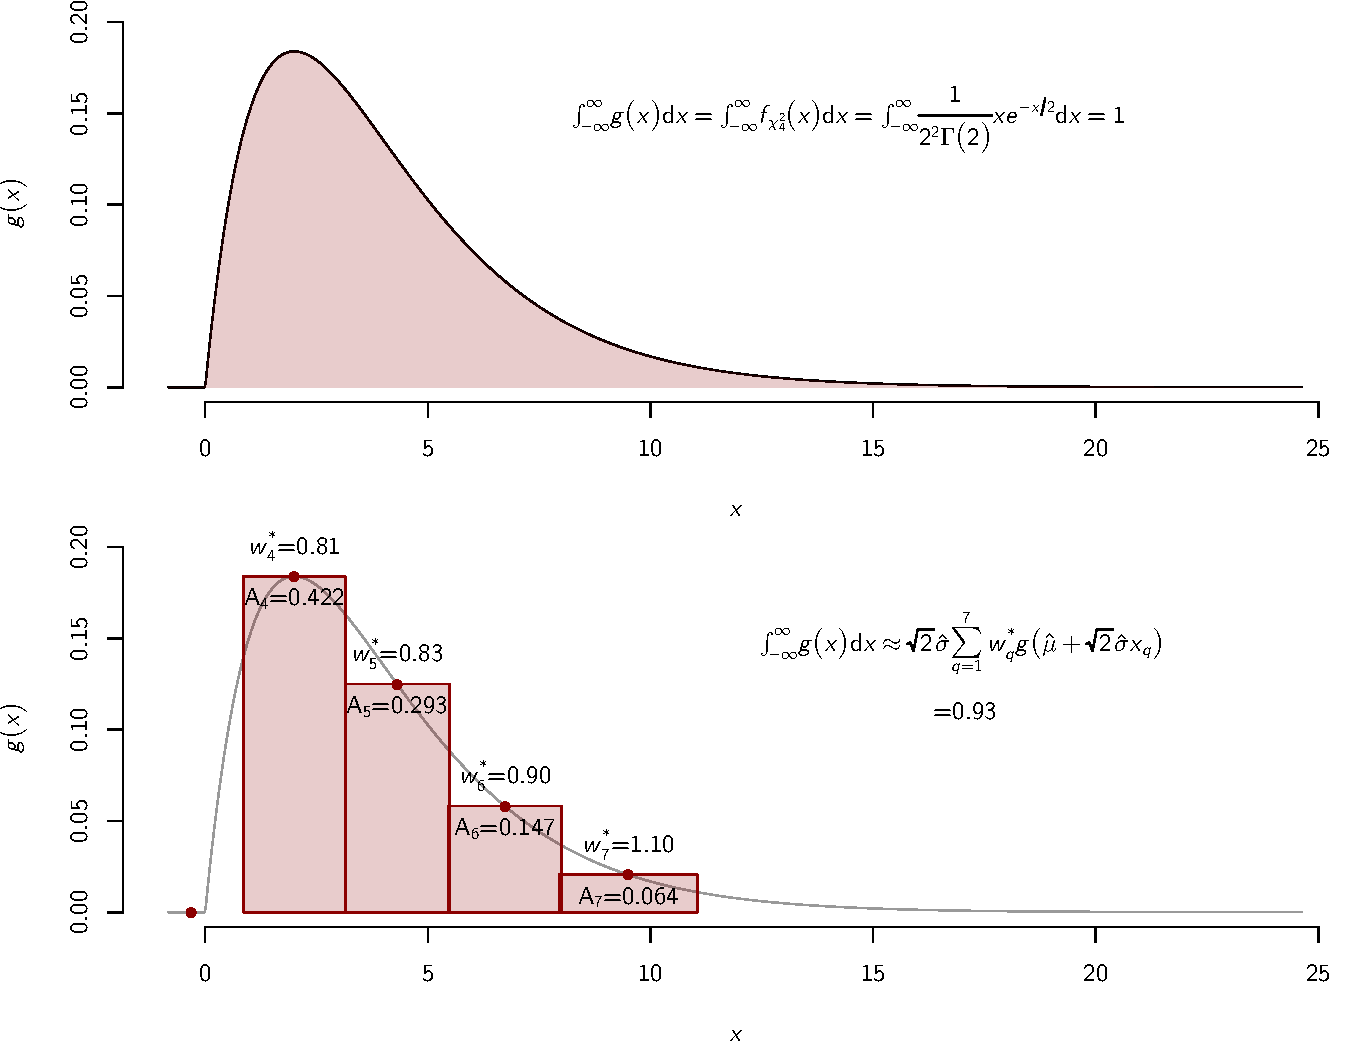
\includegraphics[width=\textwidth]{fig/g-int-example.pdf}
\end{center}

\end{frame}











%%%%%%%%%%%%%%%%%%%%% FRAME BLOCK %%%%%%%%%%%%%%%%%%%%%%

\begin{frame} %{$\tau_1$ estimates}


\begin{center}


% latex table generated in R 3.1.2 by xtable 1.7-4 package
% Thu Aug 13 18:54:52 2015

\begin{tabular}{rggccccg}
  \hline
\textcolor{lightmaroon1}{\scriptsize{$\tau_1=2$}}  & $Q=1$ & $Q=2$ & $Q=3$ & $Q=4$ & $Q=5$ & $Q=6$ & $Q=7$ \\ 
  \hline
$\alpha \left( \hat{\tau}_1 \right)$ & 0.373 & 0.954 & 0.204 & 0.035 & 0.037 & 0.040 & 0.033 \\ 
  $\bar{\hat{\tau}}_1$ & 1.671 & 1.456 & 1.757 & 1.949 & 1.927 & 2.033 & 1.990 \\ 
   \hline
\end{tabular}


\end{center}


\end{frame}



%%%%%%%%%%%%%%%%%%%%% FRAME BLOCK %%%%%%%%%%%%%%%%%%%%%%

\begin{frame}{Summary}

Statement
\begin{itemize}
\item sub statement 1
\item sub statement 2
\item sub statement 3
\end{itemize}


\end{frame}

%%%%%%%%%%%%%%%%%%%% FRAME BLOCK %%%%%%%%%%%%%%%%%%%%%%

\begin{frame}{Acknowledgements}

%{\footnotesize

Thank you to The University of Life and my co-authors.

%}


\begin{flushright} 
	
\includegraphics[height=0.1\textheight]{fig/corr.pdf}
\end{flushright}



\end{frame}







\end{document} 





%
%%%%%%%%%%%%%%%%%%%%% FRAME BLOCK %%%%%%%%%%%%%%%%%%%%%%
%
%\begin{frame}{}
%
%\end{frame}
%
%
%%%%%%%%%%%%%%%%%%%%% FRAME BLOCK %%%%%%%%%%%%%%%%%%%%%%
%
%\begin{frame}{}
%
%\end{frame}
%
%
%%%%%%%%%%%%%%%%%%%%% FRAME BLOCK %%%%%%%%%%%%%%%%%%%%%%
%
%\begin{frame}{}
%
%\end{frame}





